\documentclass[tikz,border=2pt]{standalone}
\usepackage[scaled=0.92]{helvet}
\renewcommand{\familydefault}{\sfdefault}
\usepackage[T1]{fontenc}
\usepackage{amsmath}
\usepackage{sansmath}
\sansmath
\usetikzlibrary{arrows.meta,positioning,fit,backgrounds,calc}
\definecolor{lost}{RGB}{214,96,77}      % dies with F'
\definecolor{keep}{RGB}{26,152,80}      % survives F' death
\definecolor{nv}{RGB}{49,104,176}       % survives power loss
\definecolor{ink}{RGB}{40,40,40}
\begin{document}
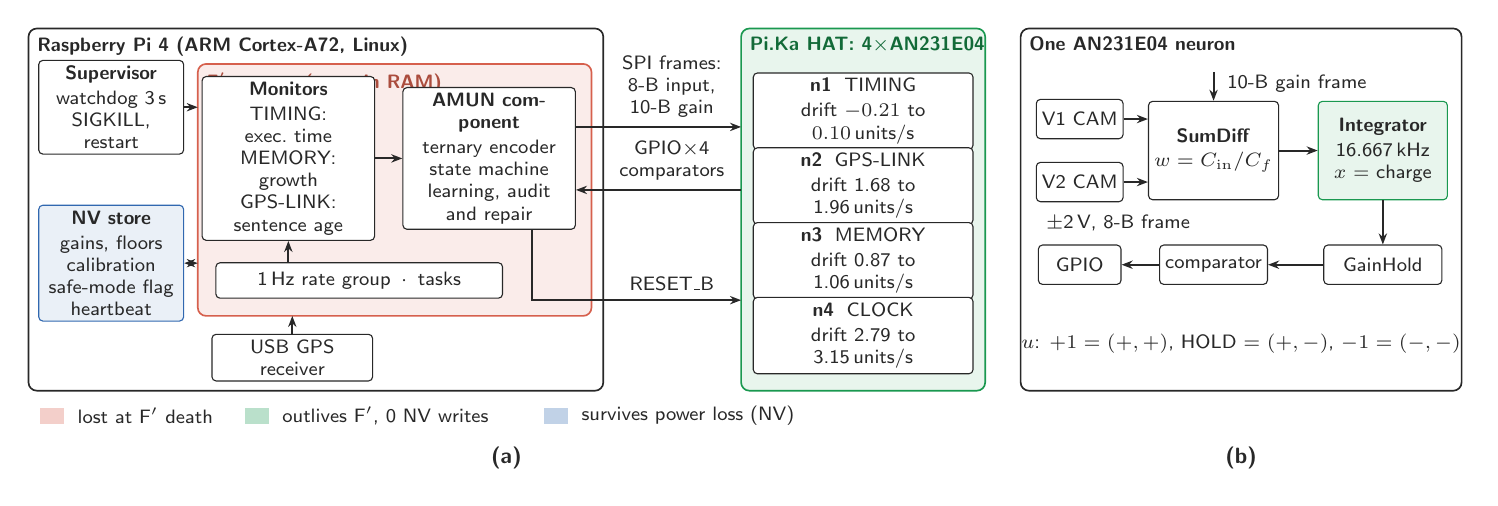
\begin{tikzpicture}[
  font=\scriptsize, ink, >={Stealth[length=4pt]},
  blk/.style={draw=ink, rounded corners=1.5pt, align=center, inner sep=2pt, fill=white},
  grp/.style={draw=ink, rounded corners=3pt, line width=0.6pt},
  ttl/.style={font=\scriptsize\bfseries, anchor=north west, inner sep=3pt},
  lnk/.style={->, line width=0.7pt},
]
% ================= (a) system =================
\draw[grp] (0,0) rectangle (7.3,4.6);
\node[ttl] at (0,4.6) {Raspberry Pi 4 (ARM Cortex-A72, Linux)};
% F' process: lost at F' death
\draw[grp, fill=lost!12, draw=lost] (2.15,0.95) rectangle (7.15,4.15);
\node[ttl, text=lost!80!black] at (2.15,4.15) {F$'$ process (state in RAM)};
\node[blk, text width=2.05cm, minimum height=1.3cm] (mon) at (3.3,2.95)
  {\textbf{Monitors}\\[1pt] TIMING: exec.\ time\\ MEMORY: growth\\ GPS-LINK: sentence age};
\node[blk, text width=2.05cm, minimum height=1.3cm] (an) at (5.85,2.95)
  {\textbf{AMUN component}\\[1pt] ternary encoder\\ state machine\\ learning, audit\\ and repair};
\node[blk, text width=3.5cm, minimum height=0.45cm] (rg) at (4.2,1.4)
  {1\,Hz rate group \,$\cdot$\, tasks};
\draw[lnk] (mon) -- (an);
\draw[lnk] (rg.north -| mon) -- (mon.south);
% supervisor and NV store (left column)
\node[blk, text width=1.7cm, minimum height=1.1cm] (sup) at (1.05,3.6)
  {\textbf{Supervisor}\\[1pt] watchdog 3\,s\\ SIGKILL, restart};
\node[blk, text width=1.7cm, minimum height=1.25cm, draw=nv, fill=nv!10] (nvi) at (1.05,1.62)
  {\textbf{NV store}\\[1pt] gains, floors\\ calibration\\ safe-mode flag\\ heartbeat};
\draw[lnk] (sup.east) -- (2.15,3.6);
\draw[lnk, <->] (nvi.east) -- (2.15,1.62);
\node[blk, text width=1.9cm, minimum height=0.4cm] (gps) at (3.35,0.42) {USB GPS receiver};
\draw[lnk] (gps.north) -- (3.35,0.95);
% PIKA HAT: survives F' death
\draw[grp, fill=keep!10, draw=keep] (9.05,0) rectangle (12.15,4.6);
\node[ttl, text=keep!70!black] at (9.05,4.6) {Pi.Ka HAT: 4$\times$AN231E04};
\foreach \i/\role/\d/\y in {1/TIMING/$-0.21$ to $0.10$/3.55, 2/GPS-LINK/1.68 to 1.96/2.6, 3/MEMORY/0.87 to 1.06/1.65, 4/CLOCK/2.79 to 3.15/0.7}{
  \node[blk, text width=2.65cm, minimum height=0.75cm] (n\i) at (10.6,\y)
    {\textbf{n\i}\; \role\\[1pt] drift \d\,units/s};
}
% links (all from the AMUN component)
\draw[lnk] (an.east |- 0,3.35) -- (9.05,3.35);
\node[above, font=\scriptsize, align=center] at (8.17,3.35) {SPI frames:\\8-B input,\\10-B gain};
\draw[lnk] (9.05,2.55) -- (an.east |- 0,2.55);
\node[above, font=\scriptsize, align=center] at (8.17,2.55) {GPIO$\times$4\\comparators};
\draw[lnk] (6.4,0 |- an.south) -- (6.4,1.15) -- (9.05,1.15);
\node[above, font=\scriptsize] at (8.17,1.15) {RESET\_B};
% legend
\begin{scope}[shift={(0.15,-0.42)}]
  \fill[lost!30] (0,0) rectangle +(0.3,0.2); \node[anchor=west, font=\scriptsize] at (0.35,0.1) {lost at F$'$ death};
  \fill[keep!30] (2.6,0) rectangle +(0.3,0.2); \node[anchor=west, font=\scriptsize] at (2.95,0.1) {outlives F$'$, 0 NV writes};
  \fill[nv!30]   (6.4,0) rectangle +(0.3,0.2); \node[anchor=west, font=\scriptsize] at (6.75,0.1) {survives power loss (NV)};
\end{scope}
\node[font=\footnotesize\bfseries] at (6.07,-0.85) {(a)};

% ================= (b) one neuron =================
\begin{scope}[shift={(12.6,0)}]
\draw[grp] (0,0) rectangle (5.6,4.6);
\node[ttl] at (0,4.6) {One AN231E04 neuron};
\node[blk, minimum width=1.05cm, minimum height=0.5cm] (v1) at (0.75,3.45) {V1 CAM};
\node[blk, minimum width=1.05cm, minimum height=0.5cm] (v2) at (0.75,2.65) {V2 CAM};
\node[blk, minimum width=1.3cm, minimum height=1.25cm] (sd) at (2.45,3.05) {\textbf{SumDiff}\\[1pt] $w=C_\mathrm{in}/C_f$};
\node[blk, text width=1.5cm, minimum height=1.25cm, fill=keep!10, draw=keep] (int) at (4.6,3.05)
  {\textbf{Integrator}\\[1pt] 16.667\,kHz\\ $x$ = charge};
\node[blk, minimum width=1.5cm, minimum height=0.5cm] (gh) at (4.6,1.6) {GainHold};
\node[blk, minimum width=1.3cm, minimum height=0.5cm] (cmp) at (2.45,1.6) {comparator};
\node[blk, minimum width=1.05cm, minimum height=0.5cm] (io) at (0.75,1.6) {GPIO};
\draw[lnk] (v1.east) -- (sd.west |- v1.east);
\draw[lnk] (v2.east) -- (sd.west |- v2.east);
\draw[lnk] (sd) -- (int);
\draw[lnk] (int) -- (gh);
\draw[lnk] (gh) -- (cmp);
\draw[lnk] (cmp) -- (io);
\draw[lnk] (2.45,4.05) -- (sd.north);
\node[font=\scriptsize, anchor=west] at (2.5,3.9) {10-B gain frame};
\node[font=\scriptsize, anchor=north west] at (0.2,2.35) {$\pm$2\,V, 8-B frame};
\node[font=\scriptsize, align=center] at (2.8,0.6)
  {$u$: $+1=(+,+)$, HOLD $=(+,-)$, $-1=(-,-)$};
\node[font=\footnotesize\bfseries] at (2.8,-0.85) {(b)};
\end{scope}
\end{tikzpicture}
\end{document}
